\documentclass[11pt]{article}
\usepackage{amsmath}
\usepackage{amsfonts}
\usepackage{graphicx} % Required for inserting images
\usepackage{tikz}
\usepackage[hidelinks]{hyperref}
\usepackage{subcaption}
\usepackage{pgfplots}
\pgfplotsset{/pgf/number format/use comma, compat=newest}
\usepackage{booktabs}
\usepackage[ruled,vlined]{algorithm2e}
	\newcommand{\ssFontBold}[1]{\textsf{\textbf{#1}}}
	\newcommand{\ssFontEmph}[1]{\textsf{\emph{#1}}}
	\SetKwSty{ssFontBold}
	\SetFuncSty{texttt}
	\SetFuncArgSty{ssFontEmph}
	\SetProgSty{ssFontEmph}
	\SetArgSty{ssFontEmph}
	\SetDataSty{sffamily}
	\SetCommentSty{texttt}
	\SetNlSty{ssFontBold}{}{}
	\SetKw{KwDownTo}{down to}
	\SetKw{KwAnd}{and}
\usepackage{microtype}
\usepackage[bottom=2.5cm, right=3.0cm, left=3.0cm, top=3.0cm]{geometry}

\title{Parallel Computing Project:\\Parallel Matrix Multiplication\footnote{Link to GitHub repository: \url{https://github.com/leonardoGemin/ParallelComputing_UniPd}}}
\author{Massimiliano Viola, 2075219 \qquad Leonardo Gemin, 2023860}
\date{}

\begin{document}

\maketitle

\section{Introduction}

Matrix multiplication is a fundamental operation in many scientific and engineering applications, like machine learning, data analysis, and signal processing to name a few. However, it is also a computationally intensive task, and parallelizing it over $P$ processors can greatly improve its performance and scalability. In this project, we study the speedup and efficiency that we can achieve with a simple parallelization strategy to multiply two $N\times N$ matrices based on scattering and broadcasting using MPI. In addition, we also evaluate the effect of further optimizations on the parallel algorithm to try to achieve even greater performance.

\section{Problem definition}

Given the two matrices $\mathbf{A}$ of size $L \times M$ \[ \mathbf{A} = \begin{pmatrix}
    a_{0,0} & a_{0,1} & \cdots & a_{0,M-1} \\
    a_{1,0} & a_{1,1} & \cdots & a_{1,M-1} \\
    \vdots  & \vdots  & \ddots & \vdots  \\
    a_{L-1,0} & a_{L-1,1} & \cdots & a_{L-1,M-1} 
\end{pmatrix} \] and $\mathbf{B}$ of size $M \times N$ \[ \mathbf{B} = \begin{pmatrix}
    b_{0,0} & b_{0,1} & \cdots & b_{0,N-1} \\
    b_{1,0} & b_{1,1} & \cdots & b_{2,N-1} \\
    \vdots  & \vdots  & \ddots & \vdots  \\
    b_{M-1,0} & b_{M-1,1} & \cdots & b_{M-1,N-1} 
\end{pmatrix} \] the matrix product $\mathbf{C} = \mathbf{A} \mathbf{B}$ is defined to be the $L \times N$ matrix \[ \mathbf{C} = \begin{pmatrix}
    c_{0,0} & c_{0,1} & \cdots & c_{0,N-1} \\
    c_{2,0} & c_{1,1} & \cdots & c_{1,N-1} \\
    \vdots  & \vdots  & \ddots & \vdots  \\
    c_{L-1,0} & c_{L-1,1} & \cdots & c_{L-1,N-1} 
\end{pmatrix} \] such that \begin{align*}
    c_{i, j} &= a_{i, 0} b_{0, j} + a_{i, 1} + b_{1, j} + \dots + a_{i, M-1} b_{M-1, j} \\
    &= \sum_{k = 0}^{M-1} a_{i, k} b_{k, j} \qquad \left\{ \;\begin{aligned}
        &\forall i \in \{0, 1, \dots, L-1\}\\
        &\forall j \in \{0, 1, \dots, N-1\}
    \end{aligned} \right.
\end{align*}

\subsection{Naive approach}\label{naive}
The naive approach to the matrix multiplication algorithm follows straight from the definition:

\begin{algorithm}[H]
    \caption{Naive matrix multiplication}
    \label{alg:naiveMM}
    \DontPrintSemicolon
    \KwIn{$\mathbf{A}$, $L \times M$ matrix, and $\mathbf{B}$, $M \times N$ matrix}
    \KwOut{$\mathbf{C} \leftarrow \mathbf{A} \mathbf{B}$, $L \times N$ matrix}
    \Begin{
        \For{$i \gets 0$ \KwTo $L$}{
            \For{$j \gets 0$ \KwTo $N$}{
                $c_{i, j} \gets 0$\;
                \For{$k \gets 0$ \KwTo $M$}{
                    $c_{i, j} \gets c_{i, j} + \left( a_{i, k} \cdot b_{k, j} \right)$\;
                }
            }
        }
        \KwRet{$\mathbf{C}$}
    }
\end{algorithm}

It requires $L \cdot M \cdot N$ multiplications and $(M - 1) \cdot L \cdot N$ additions of scalars to compute the product of two matrices. In the worst case, when both factor matrices have sizes $N \times N$, its computational complexity is $\mathcal{O}(N^3)$.

\subsection{Just a simplification}
From now on we will only deal with square matrices of sizes $N \times N$. We will also assume for the description of the algorithm (not in the code!) that $P$ divides $N$ to avoid unnecessary heavy notation.

\section{Parallelization strategy}
The approach we choose to make these computations faster by using $P$ processors is based on the following strategy:
\begin{enumerate}
    \item One process is designated as master (e.g., process $0$ of \verb|MPI_COMM_WORLD|).
    \item The master loads the matrices $\mathbf{A}$ and $\mathbf{B}$, both of size $N\times N$.
    \item The master distributes (\verb|MPI_Scatterv|) the rows of the matrix $A$ almost equally into $P$ groups of size $N/P$ (some might have one extra row if $N$ is not a multiple of $P$) to the other processes while the entire $B$ matrix is replicated (\verb|MPI_Bcast|) in all the other processes.
    \item Each process $p \in \{0, 1, \dots, P - 1\}$ computes the product of a stripe of $\mathbf{A}$ of size $N/P \times N$, denoted as $\mathbf{A}(p)$ with $\mathbf{B}$, effectively computing $N/P$ rows of the output matrix $\mathbf{C}(p)$.
    \item The master gathers (\verb|MPI_Gatherv|) all the rows from the $P$ processors and fills in the output matrix $\mathbf{C}$, which is returned.
\end{enumerate}

A simple table can help to understand better the phases of the algorithm from the perspective of the master and the worker:
\begin{table}[ht]
    \label{masterSlave}
    \centering
    \begin{tabular}{r @{\hskip 0.375in} c @{\hskip 0.375in} l}
        \toprule
        MASTER ($p = 0$) & & ($p > 0$) WORKER \\
        \midrule
        reads $\mathbf{A}$ and $\mathbf{B}$ & 1 & - \\
        sends $\mathbf{A}(p)$ to the process $p$ & 2 & obtains $\mathbf{A}(p)$ from the master \\
        replicates $\mathbf{B}$ on each process & 3 & obtains $\mathbf{B}$ from the master \\ 
        computes $\mathbf{C}(0) \gets \mathbf{A}(0) \times \mathbf{B}$ & 4 & computes $\mathbf{C}(p) \gets \mathbf{A}(p) \times \mathbf{B}$ \\
        gathers $\mathbf{C}(p)$ from process $p$ & 5 & sends $\mathbf{C}(p)$ to the master \\
        writes $\mathbf{C}$ & 6 & - \\
    \bottomrule
    \end{tabular}
\end{table}

\subsection{Complexity analysis\label{complAnalysis}}
Differently from the sequential algorithm, now each process computes in parallel only a product of two matrices of size (roughly) $ N/P \times N$, which is $P$ times faster than a $N \times N$ product given the observations made in \ref{naive}. Therefore, excluding the effect of communication (which will be analyzed in~\ref{commratio}), we expect a complexity of the order $\mathcal{O}(N^3 / P)$ for the parallel algorithm, with a speedup of the order of magnitude of $P$.

\subsection{MPI functions}
There are three major MPI-related commands in our code: \verb|MPI_Scatterv|, \verb|MPI_Bcast|, and \verb|MPI_Gatherv|. In this subsection, we explain them more in detail.
\begin{itemize}
    \item The \verb|MPI_Scatterv| function distributes data from one member across all members of a group; it extends the functionality of the \verb|MPI_Scatter| function by allowing a varying count of data, as specified in the \verb|sendcounts| array, to be sent to each process. This makes it possible to handle matrices whose size is not necessarily a multiple of the number of processors, by sending blocks of $\lfloor N/P \rfloor$ or $\lfloor N/P \rfloor + 1$ rows.

    \begin{verbatim}
MPI_Scatterv(*sendbuf, *sendcounts, *displs, sendtype,
             *recvbuf, recvcount, recvtype,
             root, comm);
    \end{verbatim}
    

    \item The \verb|MPI_Gatherv| function gathers variable data from all members of a group to one member; it extends the functionality of the \verb|MPI_Gather| function by allowing a varying count of data from each process. Again, this makes it possible to handle matrices whose size is not necessarily a multiple of the number of processors. 

    \begin{verbatim}
MPI_Gatherv(*sendbuf, sendcount, sendtype,
            *recvbuf, *recvcounts, *displs, recvtype,
            root, comm);
    \end{verbatim}


    \item The \verb|MPI_Bcast| function replicates data from one member of a group (in our case, the master process) to all members of the group.

    \begin{verbatim}
MPI_Bcast(*buffer, count, datatype,
          root, comm);
    \end{verbatim}
\end{itemize}
    

\section{Experiments}
To test the goodness of our algorithm, we performed various tests, measuring the performances of the code as the size of the matrices and the number of processors varied. To obtain coherent measurements, all the tests were carried out on the CAPRI\footnote{https://capri.dei.unipd.it/} server, whose access to computing resources is regulated via the SLURM\footnote{https://slurm.schedmd.com/overview.html} scheduler.

The variables we have taken into account are
\begin{itemize}
     \item the size of the matrices: 256, 512, 1024, 2048;
     \item the number of processors: 1, 2, 4, 8, 16.
\end{itemize}

For each setup (matrices size and number of processors in use), 10 runs were performed in order to obtain a reliable average of the measurements made. Furthermore, again for each setup, 3 variants of the code have been introduced which we will illustrate below. Finally, each of these setups has been compiled with \verb|-O3| optimization option of \verb|mpicc|. This increases the compilation time but gives important performance gains to the generated code. For consistency, also the sequential baseline has been compiled with the \verb|-O3| of \verb|gcc|.

\subsection{Three variants of the same algorithm}
Initially, the code was written using matrices (i.e. \verb|M_TYPE a[SIZE][SIZE];|\footnote{\texttt{M\_TYPE} is defined in our source code as \texttt{unsigned int}. This was done to be able to quickly change the \texttt{DATA\_TYPE} of all the variables involved. In the header of our source code there are other definitions in order to make the code more flexible to \texttt{DATA\_TYPE} changes.}). Subsequently, during the testing phase, we realized that the matrices created in this way could not run at the $1024 \times 1024$ size and larger, generating a \verb|segmentation fault| exception. So we have changed the way we handle matrices: we have converted matrices into mono-dimensional arrays in row-major order (for both the sequential baseline and parallel MPI code).
\[ \mathbf{A} = \begin{pmatrix}
    a_{0,0} & a_{0,1} & \cdots & a_{0,SIZE-1} \\
    a_{1,0} & a_{1,1} & \cdots & a_{1,SIZE-1} \\
    \vdots  & \vdots  & \ddots & \vdots  \\
    a_{SIZE-1,0} & a_{SIZE-1,1} & \cdots & a_{SIZE-1,SIZE-1} 
\end{pmatrix} \]\[ \Downarrow \]\[ \mathbf{A} = \left( a_{0,0}, \dots, a_{0,SIZE-1}, a_{1,0}, \dots, a_{1,SIZE-1}, \dots, a_{SIZE-1,0}, \dots, a_{SIZE-1,SIZE-1} \right)\]
This was made through \verb|M_TYPE *a = malloc(SIZE * SIZE * sizeof(M_TYPE))|; in this way, \verb|a[i][j]| is now accessible through \verb|a[(i * SIZE) + j]|. Note that \verb|malloc()| returns an initially null array, so it is not necessary to enter \verb|c[i][j] = 0| before performing the matrix multiplication.

\subsubsection{First variant}
The first variant, called ``mono'' in the figures, is the parallelized version of the naive approach. 

\begin{verbatim}
for (i = 0; i < sendcount / SIZE; i++)
    for (j = 0; j < SIZE; j++)
        for (k = 0; k < SIZE; k++)
            sendbuf[(i * SIZE) + j] += recvbuf[(i * SIZE) + k] 
                                     * b[(k * SIZE) + j];
\end{verbatim}
where \verb|recvbuf| and \verb|sendbuf| are, respectively, the chunks of matrices $\mathbf{A}$ and $\mathbf{C}$ destined to the current process, while \verb|sendcount / SIZE| is the number of rows of the these chunks.

\subsubsection{Second variant}
The first improvement was to transpose the matrix $\mathbf{B}$ before making it available to all processes via the \verb|MPI_Bcast()| instruction. In this way, it is possible to access both the $\mathbf{A}$ and $\mathbf{B}$ matrices row-wise and to decrease the cache misses due to the column-wise reading of the $\mathbf{B}$ matrix. In the figures, this variant has been called ``mono + transposed''.

\begin{verbatim}
for (i = 0; i < SIZE; i++)
    for (j = 0; j < SIZE; j++)
        bT[(j * SIZE) + i] = b[(i * SIZE) + j];
[...]
for (i = 0; i < sendcount / SIZE; i++)
    for (j = 0; j < SIZE; j++)
        for (k = 0; k < SIZE; k++)
            sendbuf[(i * SIZE) + j] += recvbuf[(i * SIZE) + k] 
                                     * bT[(j * SIZE) + k];
\end{verbatim}

\subsubsection{Third variant}
The last improvement, called ``mono + $k - i - j$'' in the figures, was to change the order of the three loops: instead of $i - j - k$ we adopt the $k - i - j$ order. In this way $a_{i,k}$ (better to say \verb|recvbuf[(i * SIZE) + k]|) is constant in the inner loop, while $\mathbf{B}$ and $\mathbf{C}$ (better to say \verb|sendbuf|) are scanned in row-wise. 

\begin{verbatim}
for (k = 0; k < SIZE; k++)
    for (i = 0; i < sendcount / SIZE; i++)
        for (j = 0; j < SIZE; j++)
            sendbuf[(i * SIZE) + j] += recvbuf[(i * SIZE) + k] 
                                     * b[(k * SIZE) + j];
\end{verbatim}
Note that with this method it is not necessary to transpose matrix $\mathbf{B}$. 

\newpage
\section{Results}
We analyze and plot four important performance metrics: execution time, speedup, scalability, and computing over communicating ratio. This will give a general overview of the behavior of our proposed solutions.

\subsection{Execution time}

We run the sequential baseline and the first variant of the parallel algorithm (equal in nature for comparison, with the latter just executed in parallel) on matrices of sizes 256, 512, 1024, and 2048. We observe in Fig.~\ref{fig:times} that once the algorithm and the number of processors are fixed, both the sequential and parallel algorithm scale compatibly to a cubic law, as expected. Similar patterns hold for the other algorithms as well. The line with label $N^3$ represents the reference trend in the log scale graph.

\begin{figure}[ht]
     \centering
        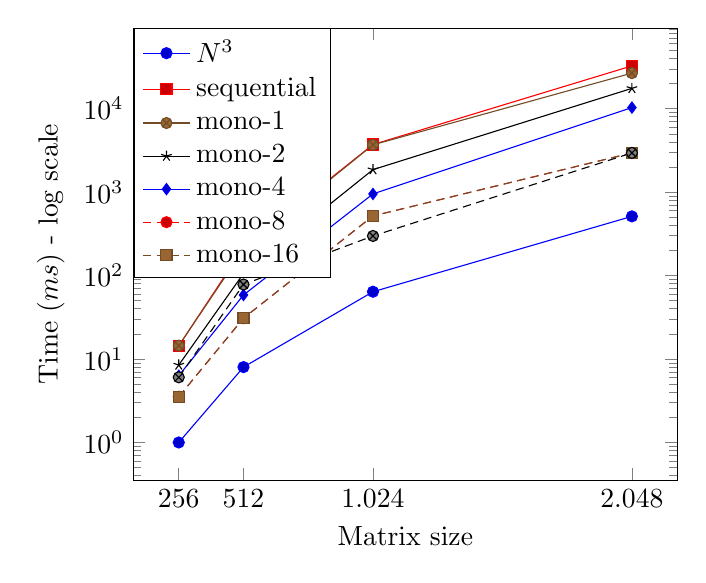
\begin{tikzpicture}
            \begin{axis}[xtick={256, 512, 1024, 2048}, xlabel={Matrix size}, ylabel={Time ($ms$) - log scale}, width=0.7\textwidth, legend style={at={(0,1)}, anchor=north west, legend cell align=left}, ymode=log,]
                \addplot coordinates {(256, 1) (512, 8) (1024, 64) (2048, 512)};
                \addplot coordinates {(256, 14.3767) (512, 215.7255) (1024, 3716.134) (2048, 32554.0933)};
                \addplot coordinates {(256, 14.459) (512, 204.465) (1024, 3685.271) (2048, 26667.156)};
                \addplot coordinates {(256, 8.474) (512, 105.856) (1024, 1859.374) (2048, 17507.209)};
                \addplot coordinates {(256, 6.299) (512, 58.485) (1024, 951.245) (2048, 10297.204)};
                \addplot coordinates {(256, 3.528) (512, 30.848 ) (1024, 518.116) (2048, 2947.842)};
                \addplot coordinates {(256, 3.528) (512, 30.848 ) (1024, 518.116) (2048, 2947.842)};
                \addplot coordinates {(256, 6.037) (512,  78.171) (1024,298.265) (2048, 2947.842)};
                
                \legend{$N^3$, sequential, mono-1, mono-2, mono-4, mono-8, mono-16}
            \end{axis}
    \end{tikzpicture}
    
    \caption{Matrix size vs execution time for the sequential and parallel matrix multiplication algorithms (with an increasing number of processors).}
    \label{fig:times}
\end{figure}

\subsection{Speedup}
The basic complexity of the algorithm, that is by executing the program without parallelizing the code ($P = 1$), is proportional to the cube of the side of the matrices: $\mathcal{O}(N^3)$. We can therefore say, up to a constant factor, that $T_{base} = N^3$.

Taking advantage of parallelization, we can increase the number of processors that will share the work to lower the execution time. With $P$ processors, as mentioned in section~\ref{complAnalysis}, the complexity per worker is reduced to $\mathcal{O}(N^3/P)$, from which $T(P) = N^3 / P$ roughy derives. We are now able to calculate the speedup factor: \begin{equation*}
    S(P) = \frac{T_{base}}{T(P)} = \frac{N^3}{N^3 / P} = P
\end{equation*}
which is optimal in theory. But let's see the behavior in practice. In Fig.~\ref{fig:performances} we see the execution time for all three parallel algorithms on all input sizes. We should see the execution time decreasing by a factor of 2 every time we double the number of processors, independently of the input size. This doesn't happen for the smaller sizes, but the pattern seems to improve the more we increase the size and give meaningful work to more processors.

\begin{figure}[h!]
    \centering
    \subcaptionbox{Matrices of sizes $256 \times 256$\label{subfig:256}}{
        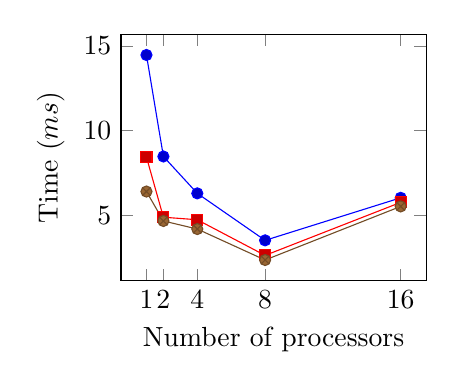
\begin{tikzpicture}
            \begin{axis}[xtick={1,2,4,8,16}, xlabel={Number of processors}, ylabel={Time ($ms$)}, width=.45\textwidth]
                \addplot coordinates {(1, 14.459) (2, 8.474) (4, 6.299) (8, 3.528) (16, 6.037)};
                \addplot coordinates {(1, 8.440) (2, 4.893) (4, 4.743) (8, 2.641) (16, 5.767)};
                \addplot coordinates {(1, 6.406) (2, 4.671) (4, 4.195) (8, 2.369) (16, 5.529)};
                %\legend{mono, mono + transpose, mono + $k-i-j$}
            \end{axis}
        \end{tikzpicture}
    }
    \hspace{\fill}
    \subcaptionbox{Matrices of sizes $512 \times 512$\label{subfig:512}}{
        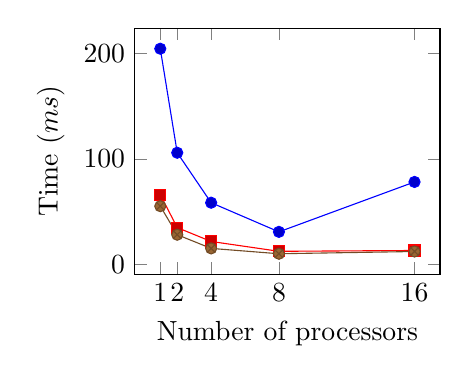
\begin{tikzpicture}
            \begin{axis}[xtick={1,2,4,8,16}, xlabel={Number of processors}, ylabel={Time ($ms$)}, width=.45\textwidth]
                \addplot coordinates {(1, 204.465) (2, 105.856) (4, 58.485) (8, 30.848) (16, 78.171)};
                \addplot coordinates {(1, 66.150) (2, 34.875) (4, 21.736) (8, 12.405) (16, 13.190)};
                \addplot coordinates {(1, 55.201) (2, 28.141) (4, 15.168) (8, 10.094) (16, 12.231)};
                %\legend{mono, mono + transpose, mono + $k-i-j$}
            \end{axis}
        \end{tikzpicture}
    }

    \vspace{2em}
    
    \subcaptionbox{Matrices of sizes $1024 \times 1024$\label{subfig:1024}}{
        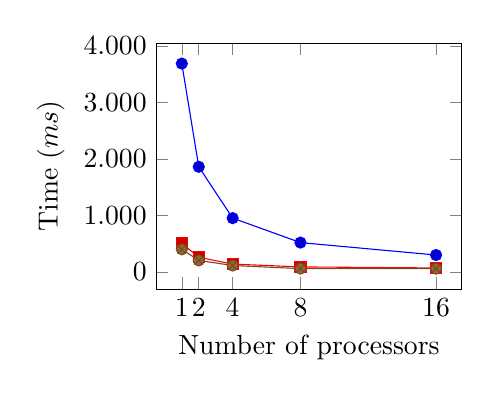
\begin{tikzpicture}
            \begin{axis}[xtick={1,2,4,8,16}, xlabel={Number of processors}, ylabel={Time ($ms$)}, width=.45\textwidth]
                \addplot coordinates {(1, 3685.271) (2, 1859.374) (4, 951.245) (8, 518.116) (16, 298.265)};
                \addplot coordinates {(1, 505.715) (2, 258.655) (4, 138.019) (8, 87.751) (16, 69.553)};
                \addplot coordinates {(1, 399.272) (2, 203.097) (4, 112.337) (8, 58.396) (16, 57.602)};
                %\legend{mono, mono + transpose, mono + $k-i-j$}
            \end{axis}
        \end{tikzpicture}
    }
    \hspace{\fill}
    \subcaptionbox{Matrices of sizes $2048 \times 2048$\label{subfig:2048}}{
        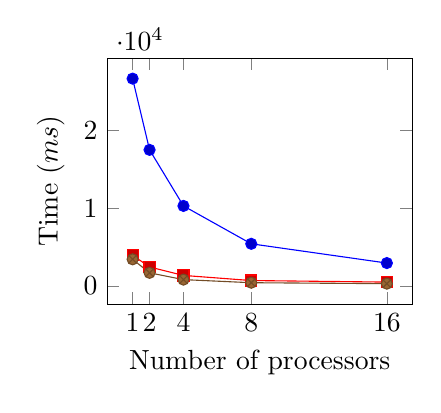
\begin{tikzpicture}
            \begin{axis}[xtick={1,2,4,8,16}, xlabel={Number of processors}, ylabel={Time ($ms$)}, width=.45\textwidth]
                \addplot coordinates {(1, 26667.156) (2, 17507.209) (4, 10297.204) (8, 5423.587) (16, 2947.842)};
                \addplot coordinates {(1, 3953.853) (2, 2441.853) (4, 1357.600) (8, 700.362) (16, 501.053)};
                \addplot coordinates {(1, 3428.401) (2, 1692.129) (4, 818.364) (8, 419.661) (16, 298.520)};
                %\legend{mono, mono + transpose, mono + $k-i-j$}
            \end{axis}
        \end{tikzpicture}
    }

    \vspace{2em}

    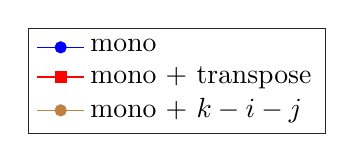
\begin{tikzpicture} 
        \begin{axis}[hide axis, xmin=10, xmax=50, ymin=0, ymax=0.4, legend style={draw=white!15!black,legend cell align=left}]
            \addlegendimage{blue,mark=*}
            \addlegendentry{mono};
            \addlegendimage{red,mark=square*}
            \addlegendentry{mono + transpose};
            \addlegendimage{brown,mark=*}
            \addlegendentry{mono + $k - i - j$};
        \end{axis}
    \end{tikzpicture}
    
    \caption{Execution time of parallel matrix multiplication algorithm, divided by size and with increasing number of processors. Lower is better.}
    \label{fig:performances}
\end{figure}

By changing the point of view and normalizing each execution time by the base time given by 1 processor for the specific algorithm according to the formula $\displaystyle{S(P) = \frac{T_{base}}{T(P)}}$, we can directly plot the speedup factors and the reference theoretical linear speedup of $P$.

\begin{figure}[h!]
    \centering
    \subcaptionbox{Matrices of sizes $256 \times 256$}{
        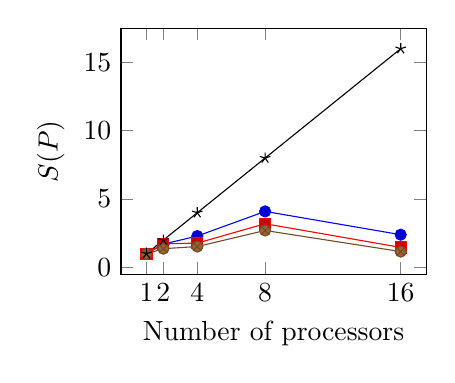
\begin{tikzpicture}
            \begin{axis}[xtick={1,2,4,8,16}, xlabel={Number of processors}, ylabel={$S(P)$}, width=.45\textwidth]
                \addplot coordinates {(1, 14.459/14.459) (2, 14.459/8.474) (4, 14.459 / 6.299) (8, 14.459 / 3.528) (16, 14.459 /6.037)};
                \addplot coordinates {(1, 8.440/8.440) (2, 8.440/4.893) (4, 8.440/4.743) (8, 8.440/2.641) (16, 8.440/5.767)};
                \addplot coordinates {(1, 6.406/6.406) (2, 6.406/4.671) (4, 6.406/4.195) (8, 6.406/2.369) (16, 6.406/5.529)};
                \addplot coordinates {(1, 1) (2, 2) (4, 4) (8, 8) (16, 16)};
                %\legend{mono, mono + transpose, mono + $k-i-j$}
            \end{axis}
        \end{tikzpicture}
    }
    \hspace{\fill}
    \subcaptionbox{Matrices of sizes $512 \times 512$}{
        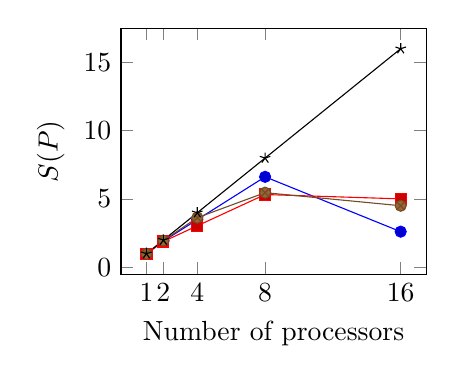
\begin{tikzpicture}
            \begin{axis}[xtick={1,2,4,8,16}, xlabel={Number of processors}, ylabel={$S(P)$}, width=.45\textwidth]
                \addplot coordinates {(1, 204.465/204.465) (2, 204.465/105.856) (4, 204.465/58.485) (8, 204.465/30.848) (16, 204.465/78.171)};
                \addplot coordinates {(1, 66.150/66.150) (2, 66.150/34.875) (4, 66.150/21.736) (8, 66.150/12.405) (16, 66.150/13.190)};
                \addplot coordinates {(1, 55.201/55.201) (2, 55.201/28.141) (4, 55.201/15.168) (8, 55.201/10.094) (16, 55.201/12.231)};
                \addplot coordinates {(1, 1) (2, 2) (4, 4) (8, 8) (16, 16)};
                %\legend{mono, mono + transpose, mono + $k-i-j$}
            \end{axis}
        \end{tikzpicture}
    }

    \vspace{2em}
    
    \subcaptionbox{Matrices of sizes $1024 \times 1024$}{
        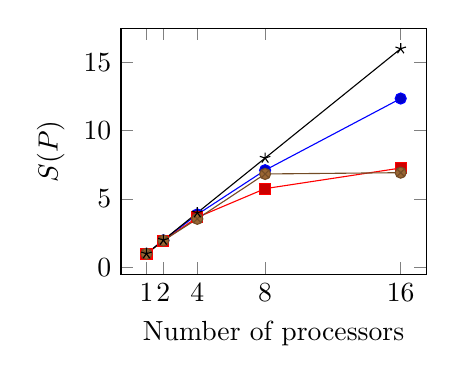
\begin{tikzpicture}
            \begin{axis}[xtick={1,2,4,8,16}, xlabel={Number of processors}, ylabel={$S(P)$}, width=.45\textwidth]
                \addplot coordinates {(1, 3685.271/3685.271) (2, 3685.271/1859.374) (4, 3685.271/951.245) (8, 3685.271/518.116) (16, 3685.271/298.265)};
                \addplot coordinates {(1, 505.715/505.715) (2, 505.715/258.655) (4, 505.715/138.019) (8, 505.715/87.751) (16, 505.715/69.553)};
                \addplot coordinates {(1, 399.272/399.272) (2, 399.272/203.097) (4, 399.272/112.337) (8, 399.272/58.396) (16, 399.272/57.602)};
                \addplot coordinates {(1, 1) (2, 2) (4, 4) (8, 8) (16, 16)};
                %\legend{mono, mono + transpose, mono + $k-i-j$}
            \end{axis}
        \end{tikzpicture}
    }
    \hspace{\fill}
    \subcaptionbox{Matrices of sizes $2048 \times 2048$}{
        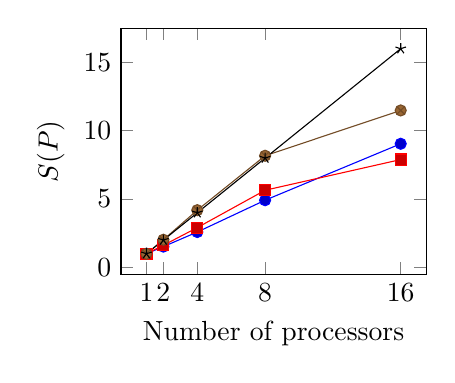
\begin{tikzpicture}
            \begin{axis}[xtick={1,2,4,8,16}, xlabel={Number of processors}, ylabel={$S(P)$}, width=.45\textwidth]
                \addplot coordinates {(1, 26667.156/26667.156) (2, 26667.156/17507.209) (4, 26667.156/10297.204) (8, 26667.156/5423.587) (16, 26667.156/2947.842)};
                \addplot coordinates {(1, 3953.853/3953.853) (2, 3953.853/2441.853) (4, 3953.853/1357.600) (8, 3953.853/700.362) (16, 3953.853/501.053)};
                \addplot coordinates {(1, 3428.401/3428.401) (2, 3428.401/1692.129) (4, 3428.401/818.364) (8, 3428.401/419.661) (16, 3428.401/298.520)};
                \addplot coordinates {(1, 1) (2, 2) (4, 4) (8, 8) (16, 16)};
                %\legend{mono, mono + transpose, mono + $k-i-j$}
            \end{axis}
        \end{tikzpicture}
    }

    \vspace{2em}

    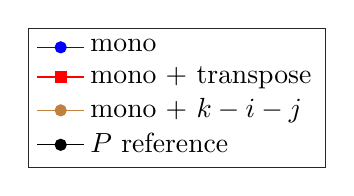
\begin{tikzpicture} 
        \begin{axis}[hide axis, xmin=10, xmax=50, ymin=0, ymax=0.4, legend style={draw=white!15!black,legend cell align=left}]
            \addlegendimage{blue,mark=*}
            \addlegendentry{mono};
            \addlegendimage{red,mark=square*}
            \addlegendentry{mono + transpose};
            \addlegendimage{brown,mark=*}
            \addlegendentry{mono + $k - i - j$};
            \addlegendimage{black,mark=*}
            \addlegendentry{$P$ reference};
        \end{axis}
    \end{tikzpicture}
    
    \caption{Empirical speedup of parallel matrix multiplication algorithm, divided by size and with increasing number of processors, versus theoretical speedup of $P$ (black line). Closer to the line is better.}
    \label{fig:speddup}
\end{figure}

\subsection{Scalability}
As far as it concerns the scalability of our algorithms, we want to determine whether or not the speedup S($P$) given by $P$ processors always increases according to the linear law that was mentioned before.
The answer as we saw is no, and not only the scalability is sublinear, but also the trend is inverted for smaller matrices and a high number of processors (e.g. 256 and 16, or 512 and 16). We believe there is a threshold after which the work assigned to each processor is not meaningful enough to justify their use, or in other words better to use fewer processors at full power rather than executing a small number of operations on a higher number of processors.


\subsection{Computing over Communicating ratio}\label{commratio}
To analyze what could be a reason for the sublinear or even harmful speedup given by a higher number of processors, we can look at the time spent calculating vs communicating. It is clear that with more processors, each of them spends less time calculating but the communication overhead increases and impacts the performance, thus this could explain the degradation after a certain threshold.

We can divide the total execution time of our parallel algorithm into the following parts: \textit{Load}, \textit{Scatter $\mathbf{A}$}, \textit{Broadcast $\mathbf{B}$}, \textit{Compute}, \textit{Gather $\mathbf{C}$}, and \textit{Save}.
The communication time is made up of the \textit{Scatter $\mathbf{A}$}, \textit{Broadcast $\mathbf{B}$}, and \textit{Gather $\mathbf{C}$} terms, while the computing part is present in the \textit{Compute} term.
Since it is hard to measure accurately all of these quantities, we employ a simpler proxy measure given by the CPU efficiency offered by Slurm, i.e. $T_{calc}/T_{total} \%$.

\begin{figure}[ht]
    \centering
    \subcaptionbox{Matrices of sizes $256 \times 256$}{
        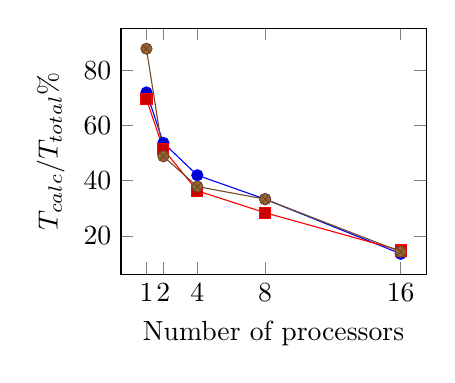
\begin{tikzpicture}
            \begin{axis}[xtick={1,2,4,8,16}, xlabel={Number of processors}, ylabel={$T_{calc}/T_{total} \%$}, width=.45\textwidth]
                \addplot coordinates {(1, 72.00) (2, 53.70) (4, 42.00) (8, 33.33) (16, 13.54)};
                \addplot coordinates {(1, 69.57) (2, 51.39) (4, 36.36) (8, 28.41) (16, 14.72)};
                \addplot coordinates {(1, 87.84) (2, 48.84) (4, 37.90) (8, 33.33) (16, 14.29)};
                %\legend{mono, mono + transpose, mono + $k-i-j$}
            \end{axis}
        \end{tikzpicture}
    }
    \hspace{\fill}
    \subcaptionbox{Matrices of sizes $512 \times 512$}{
        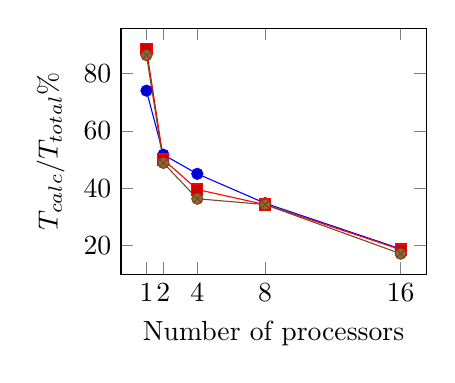
\begin{tikzpicture}
            \begin{axis}[xtick={1,2,4,8,16}, xlabel={Number of processors}, ylabel={$T_{calc}/T_{total} \%$}, width=.45\textwidth]
                \addplot coordinates {(1,  74.07)
(2,  51.67)
(4,  45.00)
(8,  34.72)
(16,  18.75)};
                \addplot coordinates {(1,  88.73)
(2,  50.00)
(4,  39.52)
(8,  34.26)
(16,  18.53)};
                \addplot coordinates {(1,  86.49)
(2,  48.81)
(4,  36.29)
(8,  34.26)
(16,  17.07)};
                %\legend{mono, mono + transpose, mono + $k-i-j$}
            \end{axis}
        \end{tikzpicture}
    }

    \vspace{2em}
    
    \subcaptionbox{Matrices of sizes $1024 \times 1024$}{
        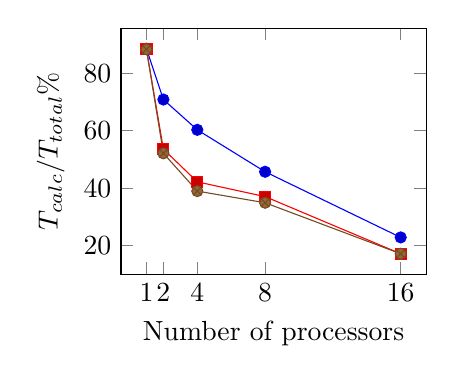
\begin{tikzpicture}
            \begin{axis}[xtick={1,2,4,8,16}, xlabel={Number of processors}, ylabel={$T_{calc}/T_{total} \%$}, width=.45\textwidth]
                \addplot coordinates {(1,  88.52)
(2,  70.83)
(4,  60.29)
(8,  45.70)
(16,  22.85)};
                \addplot coordinates {(1,  88.31)
(2,  53.57)
(4,  42.19)
(8,  37.05)
(16,  17.16)};
                \addplot coordinates {(1,  88.31)
(2,  52.11)
(4,  38.97)
(8,  34.91)
(16,  17.16)};
                %\legend{mono, mono + transpose, mono + $k-i-j$}
            \end{axis}
        \end{tikzpicture}
    }
    \hspace{\fill}
    \subcaptionbox{Matrices of sizes $2048 \times 2048$}{
        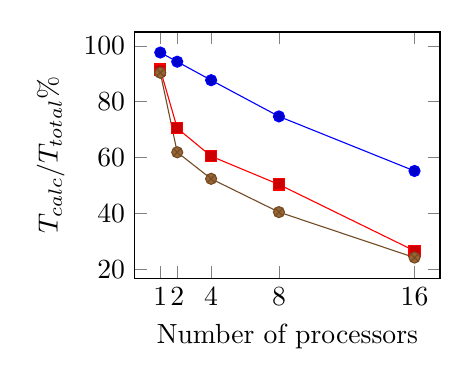
\begin{tikzpicture}
            \begin{axis}[xtick={1,2,4,8,16}, xlabel={Number of processors}, ylabel={$T_{calc}/T_{total} \%$}, width=.45\textwidth]
                \addplot coordinates {((1,  97.59)
(2,  94.31)
(4,  87.69)
(8,  74.72)
(16,  55.19)};
                \addplot coordinates {(1,  91.51)
(2,  70.49)
(4,  60.47)
(8,  50.35)
(16,  26.59)};
                \addplot coordinates {(1,  90.36)
(2,  61.88)
(4,  52.38)
(8,  40.46)
(16,  24.18)};
                %\legend{mono, mono + transpose, mono + $k-i-j$}
            \end{axis}
        \end{tikzpicture}
    }

    \vspace{2em}

    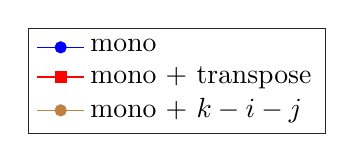
\begin{tikzpicture} 
        \begin{axis}[hide axis, xmin=10, xmax=50, ymin=0, ymax=0.4, legend style={draw=white!15!black,legend cell align=left}]
            \addlegendimage{blue,mark=*}
            \addlegendentry{mono};
            \addlegendimage{red,mark=square*}
            \addlegendentry{mono + transpose};
            \addlegendimage{brown,mark=*}
            \addlegendentry{mono + $k - i - j$};
        \end{axis}
    \end{tikzpicture}
    
    \caption{CPU Efficiency of parallel matrix multiplication algorithm, divided by size and with increasing number of processors. Higher is better.}
    \label{fig:cpueff}
\end{figure}

As we see in Fig.~\ref{fig:cpueff}, the effective computing percentage of the algorithms decreases the more processors we use, suggesting communications assume a more important role. We can notice a big waste in CPU utilization for lower sizes and a big number of processors, which is not present as severely for the largest size.

\section{Conclusion}
In this project, we coded and analyzed different variants of parallel matrix multiplication algorithms, leveraging different levels of optimization from pure parallelism over $P$ processors to reducing cache misses and doing faster loops. We also learned the importance of compiler optimization, which gave huge performance improvements just by adding the \verb|-O3| flag. As for the results, they are kind of in line with expectations: we see that for large enough matrices, increasing the number of processors leads to better execution times; for smaller matrices, using a lot of processors downgrades the performances; using more processors increases the communication time and reduces the CPU utilization.
\end{document}
